\appendix

\section{Lattice Generation} \label{apx:lattice_construction}

\begin{figure*}[t]
    \centering
    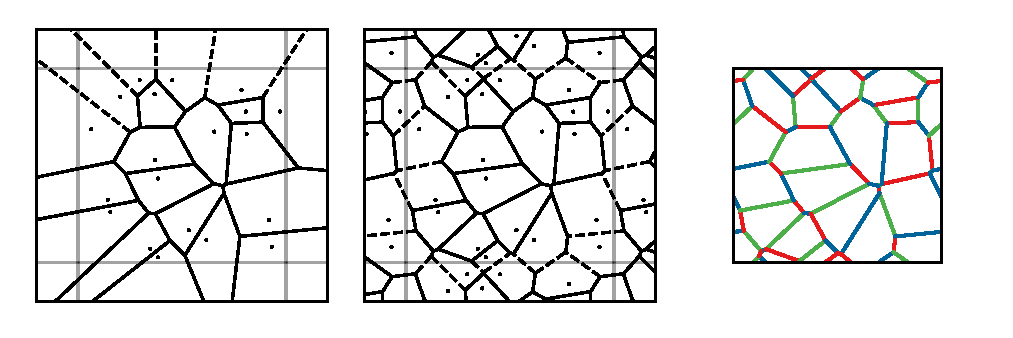
\includegraphics[width=\textwidth]{figs/lattice_construction.pdf}
    \caption{(Left) The Voronoi partition (lines) splits a region up into polyhedra closer to one of the seed points (points) than any other. In two dimensions this yields a tri-coordinate lattice. Dotted lines go off to infinity. (Center) To create a lattice on the torus, we tile the seed points into a 3x3 grid and compute a Voronoi partition. By identifying pairs of edges (dotted lines) that cross the unit square (in grey) as the same we turn this lattice into on defined on the torus. (Right) The final tri-coordinate lattice in periodic boundary conditions, coloured such that all three colours meet at every vertex.}
    \label{fig:lattice_construction}
\end{figure*}

We generate tri-coordinate lattices by taking the Voronoi partition of the unit square with respect to uniformly sampled \textit{seed points}~\cite{florescu_designer_2009}. This partitions the space into polyhedral volumes enclosing the region closest to each seed point. In two dimensions, the vertices and edges of these polygons form a tri-coordinate lattice, exactly what is necessary for the Kitaev model.
To produce lattices with periodic boundary conditions we first tile the seed points into a repeating lattice. The Voronoi partition of the tiled seed points can then be converted into a lattice embedded onto the torus by connecting corresponding edges that cross the unit square boundaries, see~\cref{fig:lattice_construction}.

Once a lattice has been generated, the bonds must be labelled in such a way that no vertex touches multiple edges of the same type, which we refer to as a \textit{three-edge colouring}. The problem of finding such a colouring is equivalent to the classical problem of four-colouring the faces, which is always solvable on a planar graph \cite{Tait1880, appelEveryPlanarMap1989a}. On the torus, a face colouring can require up to seven colours \cite{ringel_solution_1968}, so not all graphs can be assumed to be 3-edge colourable. However, such exceptions seem rare for graphs generated via voronisation -- every graph generated in this study admitted multiple distinct 3-edge colourings. In practice, the problem of finding a colouring for a given graph can be reduced to a Boolean satisfiability problem \cite{Karp1972}, which we then solve using the open-source solver \texttt{MiniSAT}~\cite{imms-sat18}.

Care must be taken in the definition of open boundary conditions, simply removing bonds from the lattice leaves behind unpaired \(b^\alpha\) operators that need to be paired in some way to arrive at fermionic modes. In order to fix a pairing we always start from a lattice defined on the torus and generate a lattice with open boundary conditions by defining the bond coupling \(J^{\alpha}_{ij} = 0\) for sites joined by bonds \((i,j)\) that we want to remove. This creates fermionic zero modes \(u_{ij}\) associated with these cut bonds which we set to 1 when calculating the projector. All our code is available online~\cite{koala}.

\section{Euler Equation and Gauge Degeneracy}
For a lattice with \(B\) bonds, \(V\) vertices, \(P\) plaquettes and genus \(g\) (1 for the torus) the Euler equation states that \(B = P + V + 2 - 2g\) which for the torus can be written as \(B = (P - 1) + (V - 1) + 2\). This corresponds nicely to the \(2^{B}\) gauge configurations being composed of \(2^{P - 1}\) physically distinct vortex states each of which is composed of \(2^{V - 1}\) gauge equivalent states that correspond to flipping three \(u_{ij}\) around a vertex. Finally there are 2 global flux operators that correspond to non-contractible loops on the torus.


\section{The Projector} \label{apx:projector}

Closely following the derivation of~\cite{pedrocchiPhysicalSolutionsKitaev2011} we can extend the projector from Majorana wavefunctions to physical spin states to the amorphous case. In the standard way, we define normal mode operators
\[(c_1, c_2... c_{2N}) Q = (b_1, b_1', b_2, b_2' ... b_{N}, b_{N}')\]
such that the Hamiltonian comes into the form
\[\tilde{H}_u = \frac{i}{2} \sum_m \epsilon_m b_m b_m'\]
from there we form fermionic operators \(f_i = \tfrac{1}{2} (b_m + ib_m')\)
and their associated number operators \(n_i = f^\dagger_i f_i\). The many body ground state within a vortex sector is then defined by the set of occupation numbers \(n_m = 0,1\). Lastly we need to define the fermion parity \(\hat{\pi} = \prod{i}^{N} (1 - 2\hat{n}_i)\).

The projector can be written as
\[ \mathcal{P} =  \mathcal{S} \left(\frac{1 + \prod_i^{2N} D_i}{2}\right) = \mathcal{S} \cdot \mathcal{P}_0\]
where \(D_i\) are the local projectors. \(\mathcal{S}\) symmetrises over gauge equivalent states while \(\mathcal{P}_0\) is responsible for annihilating unphysical states, see~\cite{pedrocchiPhysicalSolutionsKitaev2011} for details.

To extend this to the amorphous case we calculate the product of the local projectors \(D_i\)
\[\prod_i^{2N} D_i = \prod_i^{2N} b^x_i b^y_i b^z_i c_i \]
for a tri-coordinate lattice with \(N\) faces, \(2N\) vertices and \(3N\) edges. The operators can be ordered by bond type without utilising any property of the lattice.
\[\prod_i^{2N} D_i = \prod_i^{2N} b^x_i \prod_i^{2N} b^y_i \prod_i^{2N} b^z_i \prod_i^{2N} c_i\]
The product over \(c_i\) operators reduces to a determinant of the Q matrix and the fermion parity. The only problem is to compute the factors \(p_x,p_y,p_z = \pm1\) that arise from reordering the b operators such that pairs of vertices linked by the corresponding bonds are adjacent.
\[\prod_i^{2N} b^\alpha_i = p_\alpha \prod_{(i,j)}b^\alpha_i b^\alpha_j\]
This is simple the parity of the permutation from one ordering to the other and can be computed quickly with a cycle decomposition.

The final form is almost identical to the honeycomb case with the addition of the lattice structure factors \(p_x,p_y,p_z\)
\[P^0 = 1 + p_x\;p_y\;p_z \mathrm{det}(Q^u) \; \hat{\pi} \; \prod_{\{i,j\}} -iu_{ij},\] 

where \(\mathrm{det}(Q^u)\) and \(\prod u_{ij}\) depend on the lattice and the particular vortex sector. 

\section{Numerical Evidence for the Ground State Flux Sector} \label{apx:ground_state}

In this section we detail the numerical evidence collected to support the claim that, for an arbitrary lattice, a gapped ground state flux sector is found by setting the flux through each plaquette to $\phi_{\textup{g.s.}} = -(\pm i)^{n_{\textup{sides}}}$. This was done by generating a large number ($\sim$ 25,000) of lattices and exhaustively checking every possible flux sector to find the configuration with the lowest energy. We checked both the isotropic point ($J^\alpha = 1$), as well as in the toric code ($J^x = J^y = 0.25, J^z = 1$).\par
The argument has one complication: for a graph with $n_p$ plaquettes, there are $2^{n_p - 1}$ distinct flux sectors to search over, with an added factor of 4 when the global fluxes $\Phi_x$ and $\Phi_y$ wrapping around the cylinder directions are taken into account. Note that the $-1$ appears in this counting because fluxes can only be flipped in pairs. To be able to search over the entire flux space, one is necessarily restricted to looking at small system sizes -- we were able to check all flux sectors for systems with $n_p \leq 16$ in a reasonable amount of time. However, at such small system size we find that finite size effects are substantial. In order to overcome these effects we tile the system and use Bloch's theorem (a trick that we shall refer to as \textit{twist-averaging} for reasons that shall become clear) to efficiently find the energy of a much larger (but periodic) lattice. Thus we are able to suppress finite size effects, at the expense of losing long-range disorder in the lattice.\par
Our argument has three parts: First we shall detail the techniques used to exhaustively search the flux space for a given lattice. Next, we discuss finite-size effects and explain the way that our methods are modified by the twist-averaging procedure. Finally, we demonstrate that as the size of the disordered system is increased, the effect of twist-averaging becomes negligible -- suggesting that our conclusions still apply in the case of large disordered lattices. 

{\it Testing All Flux Sectors ---}
For a given lattice and flux sector, defined by $\{ u_{jk}\}$, the fermionic ground state energy is calculated by taking the sum of the negative eigenvalues of the matrix
\begin{align}
    M_{jk} = \frac{i}{2} J^{\alpha} u_{jk}.
\end{align}
The set of bond variables $u_{jk}$, which we are free to choose, determine the $\mathbb Z_2$ gauge field. However only the fluxes, defined for each plaquette according to eqn.~\ref{eqn:flux_definition}, have any effect on the energies. Thus, there is enormous degeneracy in the $u_{jk}$ degrees of freedom. Flipping the bonds along any closed loop on the dual lattice has no effect on the fluxes, since each plaquette has had an even number of its constituent bonds flipped - as is shown in the following diagram:
\begin{center}
    \input{tikzpictures/flux_loop}
\end{center}
where the flipped bonds are shown in red. In order to explore every possible flux sector using the $u_{jk}$ variables, we restrict ourselves to change only a subset of the bonds in the system. In particular, we construct a spanning tree on the dual lattice, which passes through every plaquette in the system, but contains no loops. 
\begin{center}
    \input{tikzpictures/spanning_tree}
\end{center}
The tree contains $n_p - 1$ edges, shown in red, whose configuration space has a $1:1$ mapping onto the $2^{n_p - 1}$ distinct flux sectors. Each flux sector can be created in precisely one way by flipping edges only on the tree (provided all other bond variables not on the tree remain fixed). Thus, all possible flux sectors can be accessed by iterating over all configurations of edges on this spanning tree.

\begin{figure*}[t]
    \centering
    \includegraphics[width=0.9\textwidth]{figs/appendix_diagram.png}
    \caption{(a) The energy of every flux sector explored for a system of 16 plaquettes, the order is arbitrary. The two ground state flux sectors can be identified as the points with lowest energy. (b) The fermion gap for each of the flux sectors explored. Note that the largest fermion gap coincides with the ground state flux sector. This occurred in $\sim 85\%$ of cases tested. (c) Average energy of the systems tested over a range of system sizes from $n_p$ = 9 to $n_p = 1600$. The region between the upper and lower quartiles is shown in red, and the full range of energies obtained is shown in orange. (d) Average fermion gap as a function of system size. Again, the region between the upper and lower quartiles is shown in red, and the full range is shown in orange. As can be seen, no gapless systems were found for $n_p > 20$. }
    \label{fig:energy_gaps_example}
\end{figure*}

{\it Finite Size Effects ---}
In our numerical investigation, the objective was to test as many example lattices as possible. We aim for the largest lattice size that could be efficiently solved, requiring a balance between lattice size and cases tested. Each added plaquette doubles the number of flux sectors that must be checked. 25,000 lattices containing 16 plaquettes were used. However, in his numerical investigation of the honeycomb model, Kitaev demonstrated that finite size effects persist up to much larger lattice sizes than we were able to access \cite{kitaevAnyonsExactlySolved2006}. \par 
In order to circumvent this problem, we treat the 16-plaquette amorphous lattice as a unit cell in an arbitrarily large periodic system. The bonds that originally connected across the periodic boundaries now connect adjacent unit cells. This infinite periodic Hamiltonian can then be solved using Bloch's theorem, since the larger system is diagonalised by a plane wave ansatz. For a given crystal momentum $\bf q \in [0,2\pi)^2 $, we are left with a Bloch Hamiltonian, which is identical to the original Hamiltonian aside from an extra phase on edges that cross the periodic boundaries in the $x$ and $y$ directions,
\begin{align}
    M_{jk}(\bf q) =  \frac{i}{2} J^{\alpha} u_{jk} e^{i q_{jk}},
\end{align}
where $q_{jk} = q_x$ for a bond that crosses the $x$-periodic boundary in the positive direction, with the analogous definition for $y$-crossing bonds. We also have $q_{jk} = -q_{kj}$. Finally $q_{jk} = 0$ if the edge does not cross any boundaries at all -- in essence we are imposing twisted boundary conditions on our system. The total energy of the tiled system can be calculated by summing the energy of $M(\bf q)$ for every value of $\bf q$. In practice we constructed a lattice of $50 \times 50$ values of $\bf q$ spanning the Brillouin zone. The procedure is called twist averaging because the energy-per-unit cell is equivalent to the average energy over the full range of twisted boundary conditions. \par 
{\it Evidence for the Ground State Ansatz ---}
For each lattice with 16 plaquettes, $2^{15} =$ 32,768 flux sectors are generated. In each case we find the energy (averaged over all twist values) and the size of the fermion gap, which is defined as the lowest energy excitation for any value of $\bf q$. We then check if the lowest energy flux sector aligns with our ansatz (eqn.~\ref{eqn:gnd_flux}) and whether this flux sector is gapped. \par
In the isotropic case ($J^\alpha = 1$), all 25,000 examples conformed to our guess for the ground state flux sector. A tiny minority ($\sim 10$) of the systems were found to be gapless. As we shall see shortly, the proportion of gapless systems vanishes as we increase the size of the amorphous lattice. An example of the energies and gaps for one of the systems tested is shown in fig.~\ref{fig:energy_gaps_example}. For the anisotropic phase (we used $ J^x, J^y = 0.25, J^z = 1$) the overwhelming majority of cases adhered to our ansatz, however a small minority ($\sim 0.5 \%$) did not. In these cases, however, the energy difference between our ansatz and the ground state was at most of order $10^{-6}$. Further investigation would need to be undertaken to determine whether these anomalous systems are a finite size effect due to the small amorphous system sizes used or a genuine feature of the toric code phase on such lattices. \par

{\it A Gapped Ground State ---} Now that we have collected sufficient evidence to support our guess for the ground state flux sector, we turn our attention to checking that this sector is gapped. We no longer need to exhaustively search over flux space for the ground state, so it is possible to go to much larger system size. We generate 40 sets of systems with plaquette numbers ranging from 9 to 1600. For each system size, 1000 distinct lattices are generated and the energy and gap size are calculated without phase twisting, since the effect is negligible for such large system sizes. As can be seen, for very small system size a small minority of gapless systems appear, however beyond around 20 plaquettes all systems had a stable fermion gap in the ground state. 